Vimはviから発展したテキストエディタです。コード補完、コンパイルまたエラージャンプなど、プログラミングに特化した機能が豊富です。広くプログラマに使用されています。

\begin{figure}[H]
  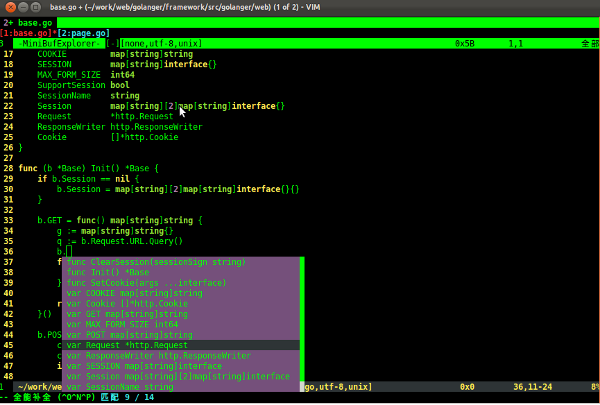
\includegraphics[width=14cm]{1.4.vim.png}
   \label{図1.9}
   \caption{VIMエディタのGoの自動補完画面}
\end{figure}


\begin{enumerate}
\item vimハイライト表示の設定
  \begin{lstlisting}[numbers=none]
cp -r $GOROOT/misc/vim/* ~/.vim/
  \end{lstlisting}
\item ~/.vimrcファイルで文法のハイライト表示を追加します
  \begin{lstlisting}[numbers=none]
filetype plugin indent on
syntax on
  \end{lstlisting}
\item Gocodeをインストールします
  \begin{lstlisting}[numbers=none]
go get -u github.com/nsf/gocode
  \end{lstlisting}
  gocodeはデフォルトで\texttt{\$GOPATH\//bin}の下にインストールされています。
\item Gocodeを設定します。
  \begin{lstlisting}[numbers=none]
~ cd $GOPATH/src/github.com/nsf/gocode/vim
~ ./update.bash
~ gocode set propose-builtins true
propose-builtins true
~ gocode set lib-path "/home/border/gocode/pkg/linux_amd64"
lib-path "/home/border/gocode/pkg/linux_amd64"
~ gocode set
propose-builtins true
lib-path "/home/border/gocode/pkg/linux_amd64"
  \end{lstlisting}
  \begin{quote}
    gocode setの2つのパラメータの意味を説明します:

    propose-builtins:はGoのビルトイン関数を補完するかです。タイプは定数です。デフォルトはfalseで、表示しません。

    lib-path:デフォルトで、gocodeは\$GOPATH\//pkg\//\$GOOS\_\$GOARCHと\$GOROOT\//pkg\//\$GOOS\_\$GOARCHディレクトリのパッケージを検索するだけです。当然この設定には私達の外側のlibを検索できるようパスを設定することができます。
  \end{quote}
\item おめでとうございます。インストール完了です。あなたは今から\texttt{:e main.go}でGoで開発する面白さを体験することができます。
\end{enumerate}


より多くのVIMの設定は、リンク(http:\//\//monnand.me\//p\//vim-golang-environment\//zhCN\//)をご参照ください。
